\chapter{GUI Design}
\thispagestyle{plain}

This chapter describes the basic structure of the instance builder web page and the various assertions and conditions required for a well defined scheduling instance.

\section{Schematic of communication}

\section{Instance structure}
To facilitate compatibility with backend C++ code, the JavaScript instance object is converted to a JSON string. JSON (JavaScript Object Notation) is a text format that is completely language independent but uses conventions that are familiar to many different programming languages, including C, C++, Java, JavaScript, Python and others. These properties make JSON an ideal data-interchange format.

JSON is built on two universal data structures:
\begin{itemize}
\item A collection of name/value pairs. In various languages, this is realized as an object, record, struct, dictionary, hash table, keyed list, or associative array.
\item An ordered list of values. In most languages, this is realized as an array, vector, list, or sequence.
\end{itemize}
Virtually all programming languages support these structures in one form or other. In JSON, they take on these forms:

An \emph{object} is an unordered set of name/value pairs. An object begins with \{ (left brace) and ends with \}  (right brace). Each name is followed by \lstinline{:} (colon) and the name/value pairs are separated by \lstinline{,} (comma).
\section{Instance object}
\setlength{\abovedisplayskip}{1pt}
\setlength{\belowdisplayskip}{1pt}
The structure of the Instance JSON object is as shown in Figure \ref{code:Instance}. The empty arrays \lstinline{[]} for \lstinline{"Units"}, \lstinline{"States"}, \lstinline{"Tasks"}, \lstinline{"Utilities"} and \lstinline{"Orders"} in the structure contain the JSON objects as specific to the instance. \lstinline{"Name"} is a string denoting the given name for the instance. \lstinline{"Horizon"} is an integer or float. \lstinline{"isCompleteInstance"} is a boolean \lstinline{true} or \lstinline{false} value denoting if an instance is completely specified.


An instance is deemed `complete' if:
\begin{enumerate}
\item At least one valid unit
\begin{itemize}
\item Positive maximum capacity
\end{itemize}
\item At least two states
\begin{itemize}
\item Positive max capacity
\end{itemize}
\item At least one valid task
\begin{itemize}
\item Non zero processing time
\end{itemize}
\item Positive horizon and at least one state to be sold with positive price OR At least one state in demand with positive demand amount
\end{enumerate}

\begin{figure}
\begin{center}
\begin{lstlisting}
{
	"Name": "Scheduling_Instance",
	"Horizon": 8,
	"Units": [],
	"States": [],
	"Orders": [],
	"Utilities": [],
	"Tasks": [],
	"isCompleteInstance": false
}
\end{lstlisting}\end{center}•
\caption{Instance JSON}
\label{code:Instance}
\end{figure}•



\subsection{Units}
The structure of the JSON object for Units is as follows:
\begin{figure}
\begin{lstlisting}
{
	"Name": "Unit1",
	"MaximumCapacity": 100
}
\end{lstlisting}
\caption{Unit JSON object}
\end{figure}•
\subsection{States}
\begin{figure}
\begin{lstlisting}
{
	"StateName": "State1",
	"StateInitialLevel": 100,
	"StateMaxLevel": 100,
	"IsZeroWait": true,
	"IsUIS": false,
	"Price": 10
}
\end{lstlisting}
\caption{State JSON object}
\end{figure}

\subsection{Utilities}
\begin{figure}
\begin{lstlisting}
{
	"Name": "Utility1",
	"MaximumAvailability": 250
}
\end{lstlisting}
\caption{Utility JSON object}
\end{figure}

\subsection{Tasks}
\begin{figure}
\begin{lstlisting}
{
	"TaskName": "Task1",
	"CompatibleUnits": [
		{
		"UnitName": "Unit1",
		"alpha": 5,
		"beta": 1
		}
	],
	"ConsumedStates": [
		{
		"ConStateName": "State1",
		"consRatio": 1
		}
	],
	"ProducedStates": [
		{
		"ProdStateName": "State2",
		"prodRatio": 1
		}
	],
	"ConsumedUtilities": [
		{
		"ConsUtilName": "Utility1",
		"CompUnit": "Unit1",
		"gamma": 2,
		"delta": 0.2
		}
	]
}
\end{lstlisting}
\caption{Task JSON object}
\end{figure}•
\subsection{Orders}
\begin{figure}
\begin{lstlisting}
{
	"StateName": "Product1",
	"Amount": 100
}
\end{lstlisting}
\caption{Order (demand) JSON object}
\end{figure}

\section{Instance builder}
Figure \ref{fig:IBGUI} shows the elements in the instance builder GUI.
\begin{figure}[htbp]
\centering
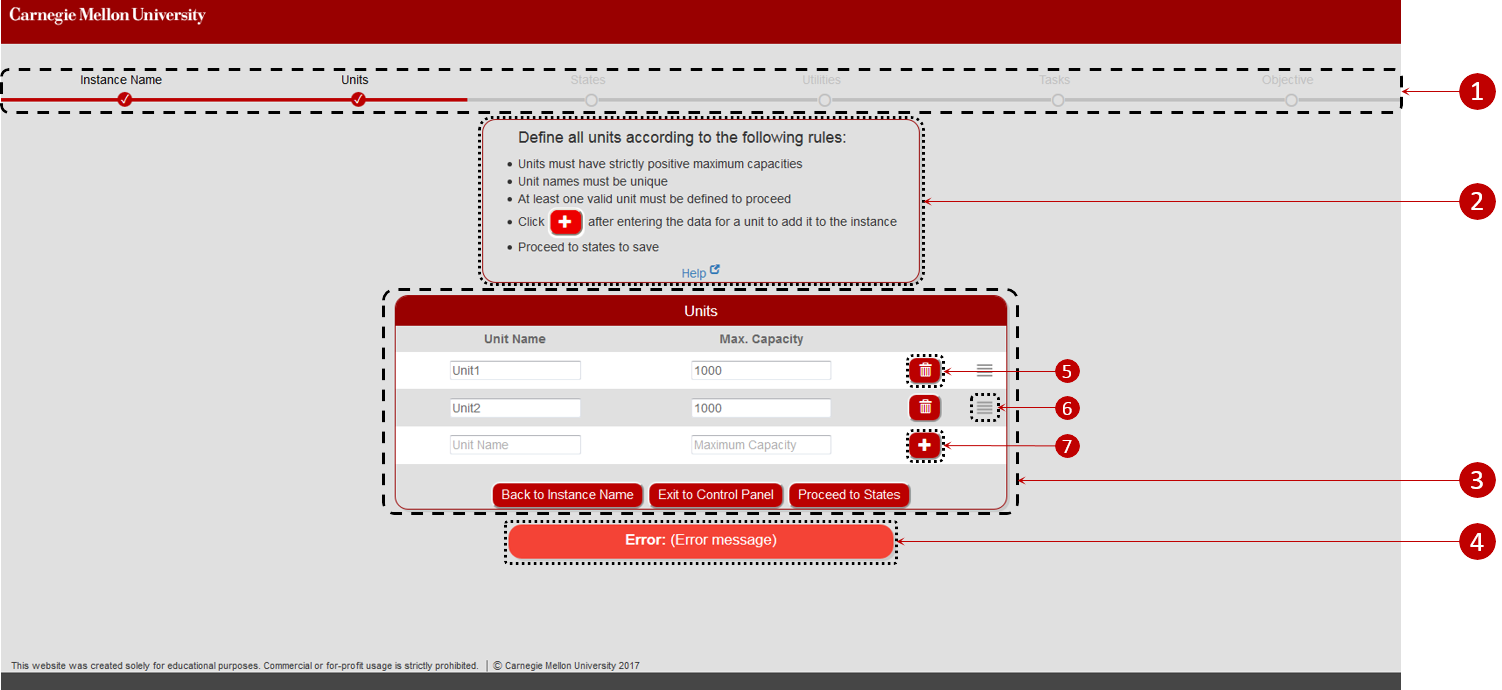
\includegraphics[width=\linewidth]{Images/GUIDesign.png}
\caption[Instance builder elements]{Instance builder elements:
1. Progress bar
2. Instructions
3. Input table
4. Error message(s)
5. Delete item 
6. Drag and drop to rearrange
7. Add new item}
\label{fig:IBGUI}
\end{figure}

\subsection{Error messages/assertions}

\subsection{List of errors}

\section{Submission page}

\subsection{Options structure}
\begin{table}[]
\centering
\caption{Uncertainty frameworks and  adjustable variables}
\label{tab:adjvars}
\begin{tabular}{@{}cccccc@{}}
\toprule
                  &            &            & \multicolumn{3}{c}{Adjustable variables} \\ \cmidrule(l){4-6} 
                  & SRO        & ARO        & \phantom{ S } T \phantom{ S}            & \phantom{ S } S \phantom{ S}           & B + S       \\ \midrule
$\alpha$          & \checkmark & \checkmark & \checkmark   & \xmark      & \checkmark  \\
$\alpha + \beta$  & \checkmark & \checkmark & \checkmark   & \xmark      & \xmark      \\
$\rho_p$          & \xmark     & \checkmark & \xmark       & \checkmark  & \xmark      \\
$\alpha + \rho_p$ & \xmark     & \checkmark & \checkmark   & \checkmark  & \xmark      \\ \bottomrule
\end{tabular}
\end{table}

\subsection{List of errors/assertions}